\documentclass[conference]{IEEEtran}
\usepackage{amsmath,amssymb,amsfonts}
\usepackage{algorithmic}
\usepackage{array}
\usepackage{tabularx}
\usepackage{graphicx}
\usepackage{textcomp}
\usepackage[backend=biber]{biblatex}
\addbibresource{ref.bib}
\usepackage{xcolor}
\usepackage{parskip}
\def\BibTeX{{\rm B\kern-.05em{\sc i\kern-.025em b}\kern-.08em
    T\kern-.1667em\lower.7ex\hbox{E}\kern-.125emX}}
\begin{document}

\title{Predicting Fetal and Maternal Health Using EHG Data\\
}

\author{
	\IEEEauthorblockN{Asya Akkus}
	\IEEEauthorblockA{\textit{Department of CDS} \\
		\textit{Case Western Reserve University}\\}
	\and
	\IEEEauthorblockN{Jakob Danninger}
	\IEEEauthorblockA{\textit{Department of CDS} \\
		\textit{Case Western Reserve University}\\}
	\and
	\IEEEauthorblockN{Stephen Tashobya}
	\IEEEauthorblockA{\textit{Department of CDS} \\
		\textit{Case Western Reserve University}\\}
	\and
	\IEEEauthorblockN{Andrew Xue}
	\IEEEauthorblockA{\textit{Department of CDS} \\
		\textit{Case Western Reserve University}\\}
	\and
	\IEEEauthorblockN{Jason Zheng}
	\IEEEauthorblockA{\textit{Department of CDS} \\
		\textit{Case Western Reserve University}\\}
}

\maketitle

\begin{abstract}
	The United States has the highest fetal and maternal mortality rates of any developed country. In 2021 alone, 1205 women died from pregnancy related deaths and the fetal mortality rate in the US has climbed by 3\% \cite{maternal}. Additionally, minorities and marginalized groups are disproportionately impacted by these statistics (2). As a result of the significant prenatal health risks and limited foresight/insight, there is a need to model parameters and information present during labor to efficiently diagnose complications and their potential consequences.
	In the course of our work, we will utilize two datasets from the Physionet repository, combining data from the “Term-Preterm EHG Database”  and the “Term-Preterm ElectroHysteroGram Dataset with Tocogram” along with clinical data collected from pregnant women during routine pregnancy checkups and from those admitted to the hospital due to threatened preterm labor.

	We will develop classification and regression models to predict a term or a preterm birth. The classification models will be trained specifically to predict categorical outcomes, i.e., delivery at term or preterm. Pursuing a different approach, we will train the regression models to predict the gestational age at delivery, labeling predictions lower than 37 completed weeks, or 259 days, as preterm, and those above 37 weeks as term. In developing the classification and regression models, we will use clinical information alone, EHG measurements alone, and clinical information combined with EHG measurements.We hypothesize that combining all the available information can improve the performance of our models.

	First, we will start by predicting preterm births by using only the clinical information, which supplements the EHG measurements. We will develop two models: a logistic regression model to determine whether a pregnancy would result in preterm birth, and a linear regression model to predict the gestational age at delivery.

	Using only the EHG measurements, we will predict whether the mothers delivered preterm or at term. We will start by preprocessing all the EHG measurements by removing the first minute of the recordings to remove transient effects. Next, we will filter the measurements to remove baseline wander and high-frequency noise. Filter techniques with zero-phase and cutoff frequencies will be considered since we are dealing with non-stationary signals.
	The processed data will then be fed into the recurrent neural network(LSTM)  cells which can learn patterns from sequential data: in our case, these cells are intended to learn patterns from the spectral changes of the EHG measurements over time.

	We will evaluate the performance of our models using a stratified cross-validation and statistical analysis based on confidence intervals and to reduce the risk of bias.
	To further assess the performance of our models, we will measure the sensitivity, positive predictive value (PPV), and negative predictive value (NPV) at various specificity levels. We include the PPV and NPV in our analysis because these statistics consider the incidence of preterm births in the dataset.

\end{abstract}

\begin{IEEEkeywords}
	machine learning, term preterm, fetal health, ehg, electrohysterogram
\end{IEEEkeywords}

\section{Introduction}
Preterm birth is a massive global issue that increases the risk of birth defects, preeclampsia, fetal mortality, and maternal mortality. The United States has the highest fetal and maternal mortality rates of any developed country. In 2021 alone, 1205 women died from pregnancy related deaths and the fetal mortality rate in the US has climbed by 3\%[1]. To make matters worse, Cuyahoga county has some of the worst birth outcomes in the state with East Cleveland having the worst birth outcomes of any city in Ohio. In addition to all the issues associated with preterm birth, predicting preterm birth remains challenging, especially in areas with scarce medical resources.
As a result of the significant prenatal health risks and limited foresight/insight, researchers have started developing different computational techniques to quickly and effectively quantify the risk of preterm birth. This could help this issue by allowing medical staff to serve more patients in a more effective way without the need for expensive new equipment. This field is still in its infancy and we hope to add to the existing literature.
We combined data from the “Term-Preterm EHG Database”  and the “Term-Preterm ElectroHysteroGram Dataset with Tocogram” along with clinical data collected from pregnant women during routine pregnancy checkups in order to develop our own pregnancy classification models. Due to having a relatively large team for the project, we decided to focus on multiple machine learning techniques in order to maximize our output. The classification models will be trained specifically to predict categorical outcomes, i.e., delivery at term or preterm. Pursuing a different approach, we will train the regression models to predict the gestational age at delivery, labeling predictions lower than 37 completed weeks, or 259 days, as preterm, and those above 37 weeks as term. In developing the classification and regression models, we will use clinical information alone, EHG measurements alone, and clinical information combined with EHG measurements.We hypothesize that combining all the available information can improve the performance of our models.

\section{Related Works}
\subsection{Predicting risk of preterm birth in singleton pregnancies using machine learning algorithms - Yu et al.}
This paper focuses on purely clinical facts in order to predict preterm and term pregnancy outcomes. This was achieved by partnering with a Chinese hospital system and collecting clinical data from about 22,000 pregnancies. Each pregnancy had multiple check ups and the main information collected from each patient was demographic, lifestyle, health history, pregnancy history, and current medical measurements. The researchers proceeded to use a CatBoost to train their prediction model. They were able to achieve an AUC of .70. This paper proves that clinical data without EHG data is highly relevant for predicting birth outcomes.

\subsection{Predicting preterm births from EHG recordings via deep learning - Goldsztejn \& Nehorai}
Goldsztejn and Nehorai use the same datasets as us to create a ML model to predict term and preterm birth. The challenge was that sometimes there is missing clinical data. In order to account for this, Goldztejn and Nehorai started by creating outcomes by processing the EHG data using a LSTM model. Then they combined the LSTM outcomes with a clinical data regression model to boost the results. If there was no clinical data available they will return the LSTM results. This was a generally effective approach and led to a AUC of .78, surpassing Yu Et Al’s clinical data only approach.

\subsection{Prediction of Preterm Labor from the Electrohysterogram Signals Based on Different Gestational Weeks - Far et al.}
This paper is similar to Goldsztejn and Nehorai but uses boosting (AdaBoost) and very intense feature engineering. This approach was very fruitful leading to an AUC of .98 which is exceptionally high. However despite the earth shattering result this paper is not well cited. Some academics criticize this paper since they did not explain how they prevented data leakage which could explain the extreme accuracy of their model.

\section{Data Description}
\subsection{Overview of the dataset}
The dataset contains electrohysterogram (EHG) recordings collected for the analysis of preterm and full-term pregnancies. The primary goal of this dataset is to identify patterns that can help in predicting preterm births using signal data. A standardized protocol was used to collect the recordings, and pre-processing techniques were used to prepare the data for analysis in order to ensure accuracy and consistency.

\subsection{Signal Recording Origins}
Both the datasets that were used had probes in the configuration seen in the diagram. The EHG signals were captured at four electrode points placed on the abdomen. The signals were measured using:
\begin{itemize}
	\item A sampling frequency of 20 Hz to 100 Hz
	\item 3 Continuous recordings from points E1 to E2, E2 to E3, and E3 to E4.
\end{itemize}
The spatial accuracy of uterine activity detection is ensured by this configuration, which is crucial for examining signal differences between preterm and full-term pregnancies.

\begin{figure}[h]
	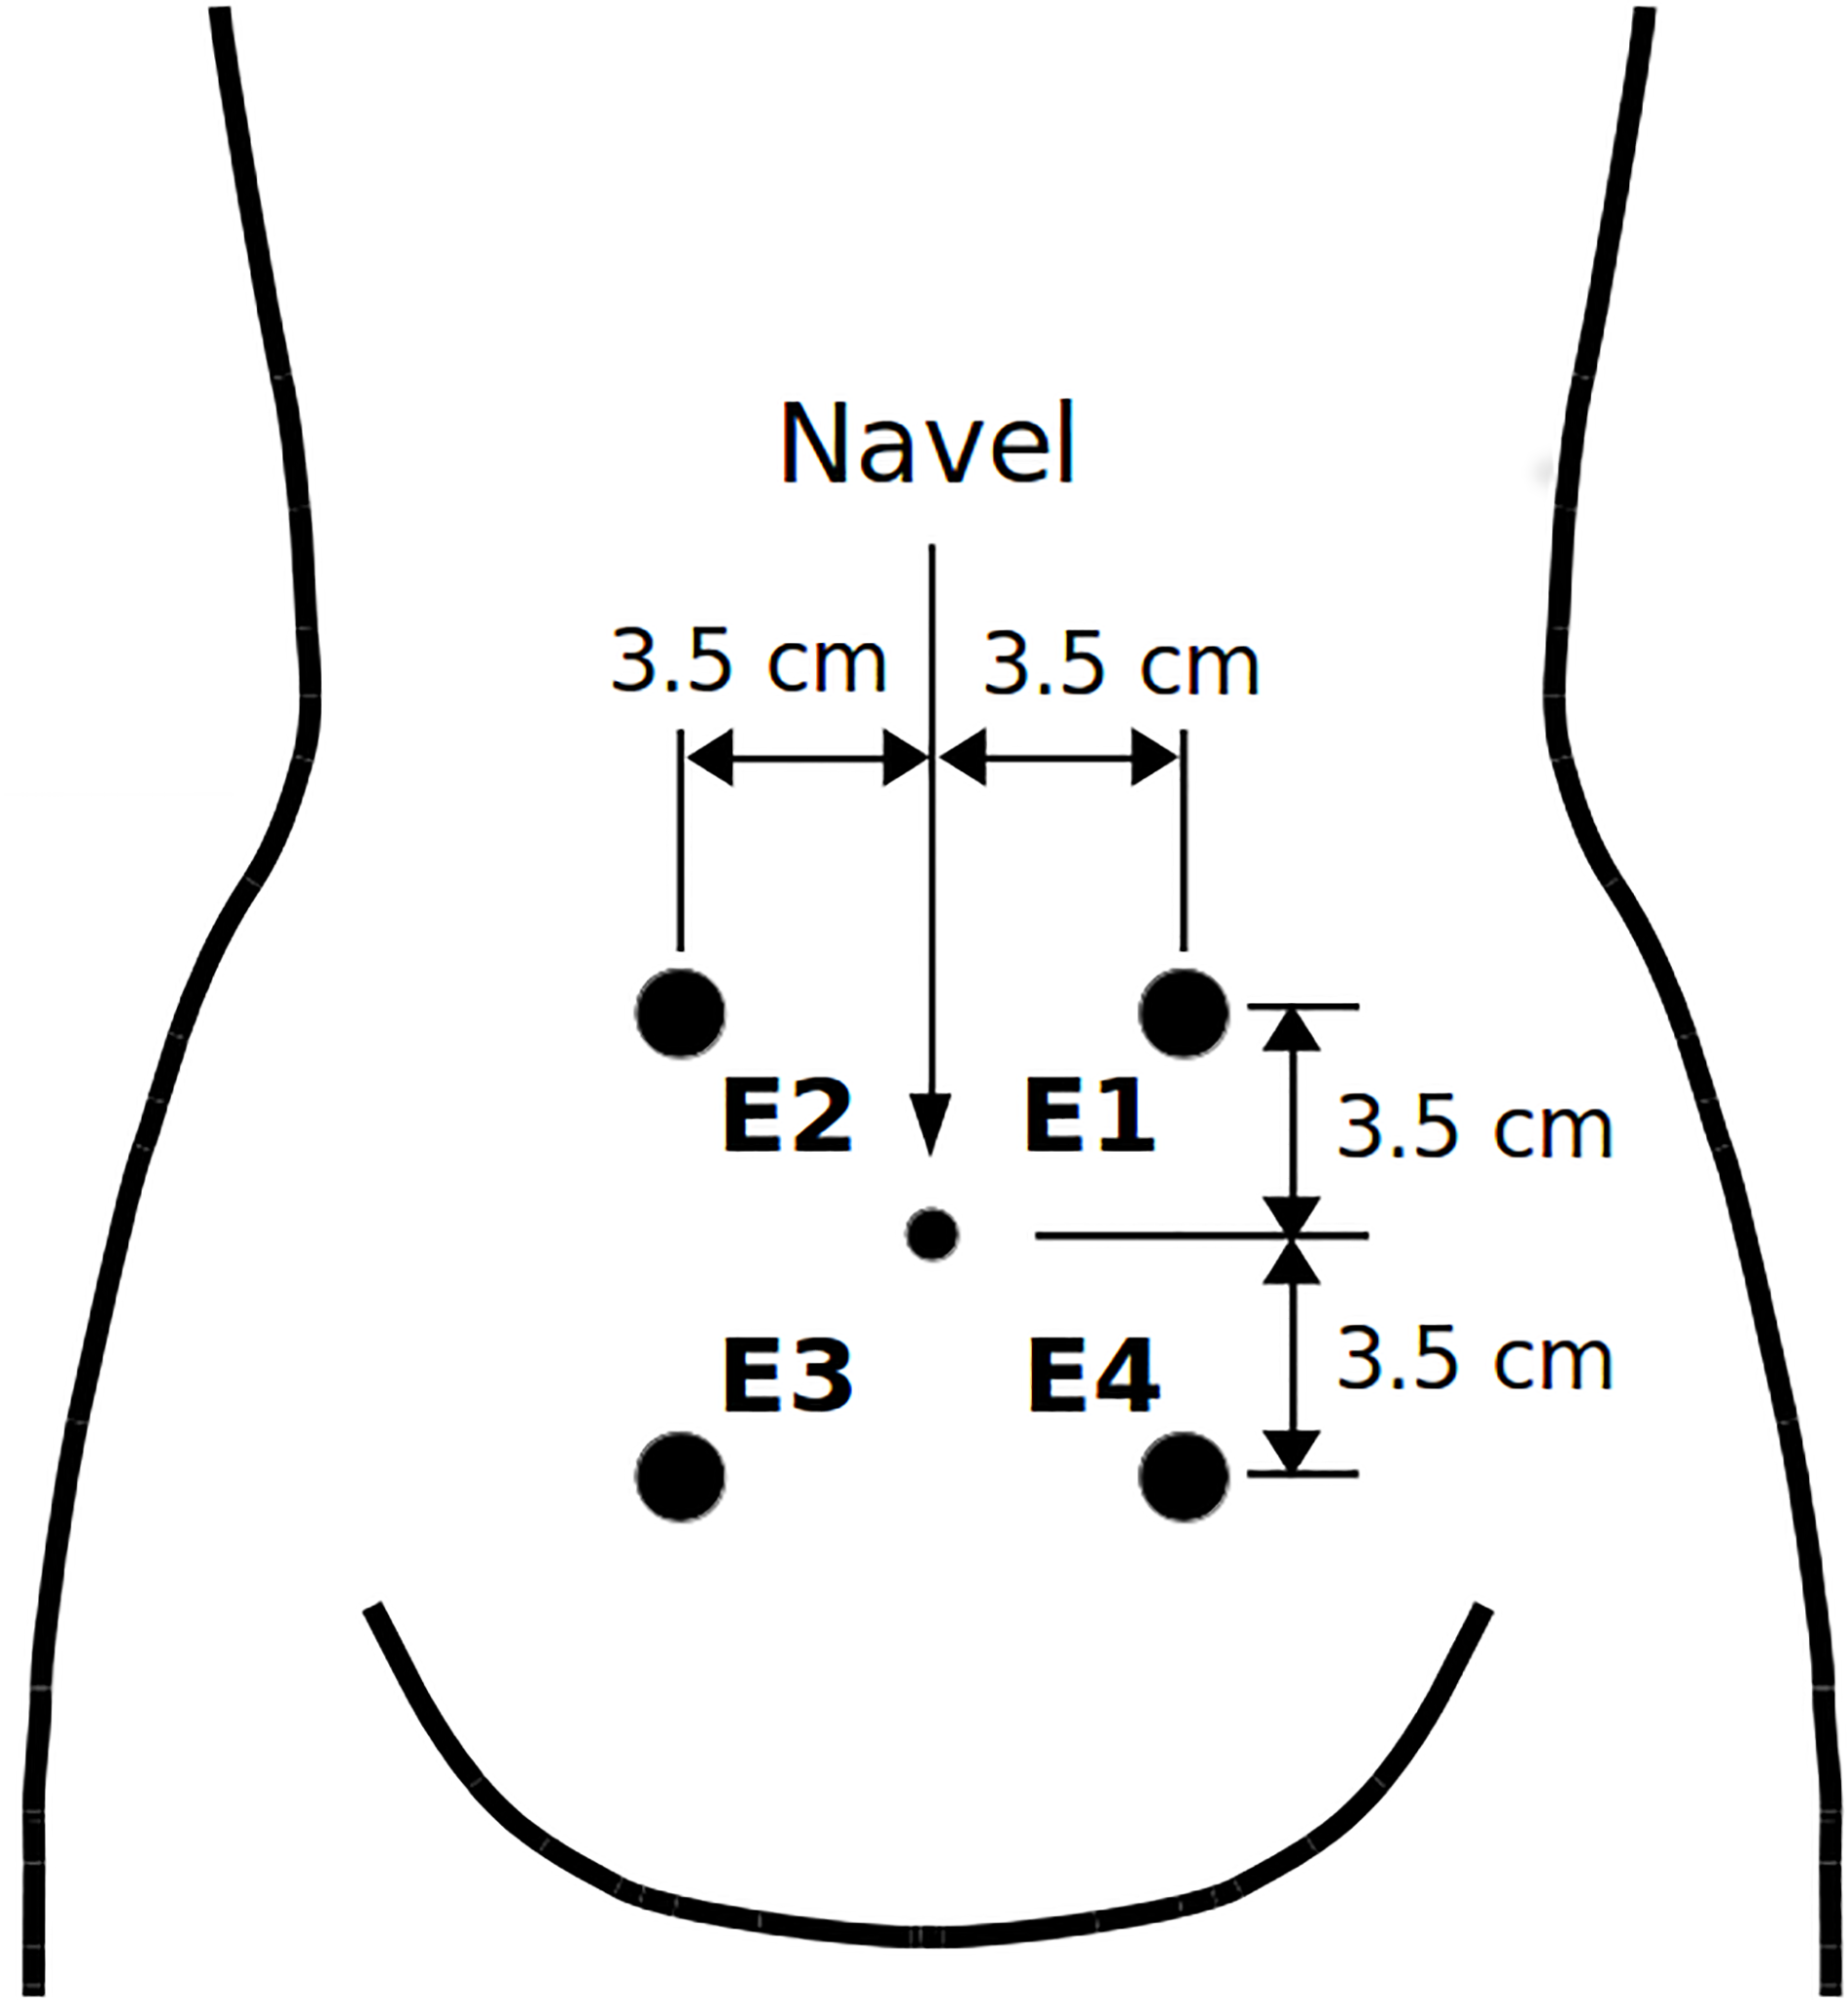
\includegraphics[width=0.5\textwidth]{images/sensor_placement.png}
\end{figure}

\subsection{Data sources}
\subsubsection{Term-Preterm EHG Database (TPEHG):}
Contains recordings from 262 women who had full-term pregnancies and 38 cases with premature pregnancies. 162 recordings were taken before the 26th week of gestation, 138 were taken after.
\subsubsection{The Term-Preterm Electrohysterogram Dataset with Tocogram (TPEHGT):}
Contains data from 31 four-signal 30 minute uterine EHG records. Of the 31 records, 13 were full-term pregnancies, 13 were premature and 5 were controlled.
Adjustments: Two recordings, originally 26 and 33 minutes long, were re-padded(zero padding the 26 minute record and truncating the 33 minute record) to fit the standardized 30-minute recording length. This is done to ensure uniformity across the dataset which ensures definitive signal analysis across all the samples.

\subsection{Statistical Dsecription of Data}
Standard Sampling Frequency: 13107Hz, with a few entries recorded at 20Hz.
A consistent channel count of 40 indicates that all signals were recorded with the same setup, enhancing comparability between the preterm and full-term groups. The data exhibits the following key statistics:

  \begin{tabularx}{0.5\textwidth} { 
  | >{\raggedright\arraybackslash}X 
  | >{\centering\arraybackslash}X 
  | >{\raggedleft\arraybackslash}X | }
    \hline
		Statistical Metric     & Sampling Frequency & Number of Channels \\
    \hline
		Count                  & 4089               & 4089               \\
    \hline
		Mean                   & 11574.76           & 36.8-              \\
    \hline
		Standard Deviation     & 4159.98            & 8.73               \\
    \hline
		Minimum                & 20                 & 8                  \\
    \hline
		25\% Quartile          & 13107              & 40                 \\
    \hline
		50\% Quartile (Median) & 13107              & 40                 \\
    \hline
		75\% Quartile          & 13107              & 40                 \\
    \hline
	\end{tabularx}
  
  \textbf{please read this and replace with those figures its 4:20 AM and I need to sleep}

\subsection{Signal Data Processing}
\subsubsection{Preprocessing}
Before conducting the analysis, several preprocessing steps were implemented to ensure data quality:
\begin{itemize}
  \item Filtering:
Signals were filtered to remove low-frequency noise, baseline drifts, and high-frequency distortions.
Specific filters that were implemented by the original research team include Butterworth low-pass filters with cutoff frequencies of 0.05 Hz (low) and 4 Hz (high).
\item Fast Fourier Transform (FFT):
FFT was used to help in identifying key spectral features that differ between preterm and full-term groups.
\item Downsampling:
The signals were downsampled to optimize computational efficiency without losing critical information.
Downsampling ensures that the model can process the data effectively while retaining signal integrity.
\end{itemize}

\subsection{Challenges and Considerations}
\begin{itemize}
  \item Imbalance in Data:
Preterm records account for only 12.7\% of the dataset, introducing a significant imbalance that can bias ML models toward predicting full-term outcomes.
\item Signal Complexity:
EHG signals are inherently noisy and vary widely across subjects due to physiological differences, requiring complex preprocessing and feature extraction.
\item Model Extrapolation:
Efforts to reduce bias and improve signal clarity ensure that the final model generalizes well across different populations.
\end{itemize}

\section{Issues Highlighted by SVM}
\subsection{Significance of Data Imbalance}
We can directly notice an imbalance in our data with 300 records provided but only 38 (12.7\%) corresponding to preterm births. But how does this imbalance affect the accuracy of machine learning models? 

Imbalance of data causes models to favor the majority class, in this case (term births) because it dominates the data set, leading to biased predictions. For example, in regards to this data set, a model could just predict term birth regardless of the input as it would be accurate 87.3\% of the time just due to the data imbalance. This would be at the expense of accurately predicting the minority class (preterm births), resulting in poor recall and precision for classifying preterm births.

\subsection{SVM Implementation and Predictions}
\subsubsection{What is a Support Vector Machine (SVM)}
A support vector machine is a machine learning algorithm that attempts to classify data by finding an optimal boundary, known as a hyperplane, that attempts to optimally separate data classes so that when future predictions are plotted they can be determined based on the hyperplane boundary. 

The algorithm works by fitting weight vectors and biases which correspond to the position and orientation of the hyperplane and identifying the support vectors as points closest to this hyperplane. The hyperplane will be gradually refined as the weights and biases are tweaked to ensure the greatest margin between the hyperplane and the closest support vectors. 

\subsubsection{Interpreting results from SVM}
The accuracy of the SVM was poor at 33\% (See figure Include the result figure and name it somewhere in appendix). The recall and precision scores in regards to the classification of the minor class (preterm births) were poor as to be expected. Further diving into this result, we notice only 12\% of preterm birth predictions made by the model were actually correct. This low precision often occurs due to the model attempting to make excessive predictions in favor of the minority class to compensate for the data imbalance, leading to many false positives. \textbf{bruh why is this not finished :(}

\subsection{Why the SVM struggled}
When given an imbalanced data set where there exists much more data regarding one classification over another, it makes it much harder for the SVM to position the decision boundary fairly. As such, the SVM tends to favor the larger team as that is what is often the correct decision during testing. This reduces the area that is classified as minority data points as they contribute less to the decision boundary. As a result, new data points from the minority class would often end up misclassified during testing.

\subsection{Addressing the imbalance}
Data imbalance is a common challenge in machine learning, particularly when working with datasets where one class significantly outnumbers another. This imbalance often results in biased models that favor the majority class as can be seen with the simple SVM above. As such, researchers have developed multiple solutions towards addressing data such as data-level approaches and machine learning algorithm level approaches. 

\section{Methodology}
Data level approaches consist of strategies such as resampling and data duplication in regards to the minority class. There even exist strategies that generate synthetic examples for the minority class by looking through existing samples. However, what is common amongst all data level strategies is that they all attempt to ensure that the proportionality between the majority class and the minority class are more equal to reduce a model’s bias.

However, even more important in dealing with class imbalance in machine learning would be selecting the right model. Some algorithms, such as Gradient Boost, Random Forests and Recurrent Neural Networks (RNNs), inherently handle class imbalance due to their flexibility and structure. As such, we have chosen to explore and compare the performance of these three machine learning models on our data set. By analyzing their performance, we aim to identify the most effective machine learning approach towards predicting term and preterm births given the data and data collection methods defined above. Our candidates for viable machine learning models are explored in the following sections.

\subsection{Gradient Boosting}
Gradient boosting is a powerful machine learning technique that combines the predictions of multiple weak models to create a strong, accurate model. It works by sequentially adding weak learners, typically decision trees, to the ensemble. Each new tree focuses on correcting the errors made by the previous models. This process continues until the desired level of accuracy is achieved or a stopping criterion is met.

Our implementation of gradient boosting includes a series of Python scripts. We first convert all of the data into CSVs. This step was done so the data would be in a format we were comfortable with and allow us to implement the data processing and GPU acceleration using our preferred methods. The waveform data for each patient was converted into a separate CSV, which was then renamed with another Python script to add reference data about the patient outcome (term, preterm, early) into the file name. Finally, the last Python script implements gradient boosting and applies it to the data. 

Our implementation of gradient boosting utilizes the XGBoost Python library. XGBoost is also known as Extreme Gradient Boosting. It is a popular, tested gradient boosting library that features CUDA acceleration with CuPy and Rapids CuML. CuPy is a drop in replacement for NumPy, making it easier to accelerate NumPy features, and in combination with CuML, we can process all of the data simultaneously. These features help us process the large amount of converted CSV data faster. In the script, our data is imported as CuPy vectors. We split 30\% of the data into a test dataset and trained the data on the remaining 70\%. Then, we ran XGBoost to create the model before testing its accuracy. 

We used area under the curve (AUC) to evaluate model accuracy because the data contains a disproportionately higher number of normal, healthy births. With a max depth of 6, an ETA of 0.3, and using a uniform sampling method, our best model, which has both a fast fourier transform and a butterworth filter applied to the data, has an AUC of 0.79. Without the fourier transform, we were able to achieve an AUC of 0.76, and without either the butterworth filter or the fourier transform, we only achieved an AUC of 0.69.  Below is a summary of the XGBoost results

\textbf{insert fig here}

XGBoost compared favorably to all other models discussed in the related works section, only bested by the model from Mohammadi Far Et Al., which includes heavy feature engineering. However, XGBoost suffers from some data leakage, so we are not entirely confident that these figures accurately represent the performance of our model.

\subsection{Random Forests Classification and Regression}
Random Forest is an ensemble learning method that utilizes multiple decision trees for both regression and classification tasks. It works by employing bootstrap sampling and random feature selection. Bootstrapping is the action of creating random subsets of the training data with replacement to train each decision tree independently. Random feature selection is employed at each split in the decision tree, where a random subset of features is considered instead of using all available features. This helps to reduce overfitting and improve generalization. In classification tasks, the final output is determined through majority voting across all trees. In regression tasks, on the other hand, the result is obtained by averaging the outputs of all trees. The key distinction between the Random Forest Classifier and Regressor lies in their application. The classifier is used for problems with discrete labels, whereas the regressor is suited for continuous outputs. This combination of randomness and ensemble decision-making makes Random Forest a robust and versatile model that is a good candidate for the datasets used in this study when it comes to their classification and further extrapolation of one feature from all the others. 
Scikit-learn (Sklearn) is a popular library in Python that is typically utilized for building machine learning projects. For this study, it provides the Random Forest algorithm through classes like RandomForestClassifier and RandomForestRegressor, as well as utilities such as the train\_test\_split method for data management. While a useful start to making scalable machine learning systems, Sklearn relies solely on CPU computation. This can limit scalability for very large datasets. As a result, tools like CUDA, DASK, and ParallelPostFit address this limitation by harnessing GPU power. GPU parallelization accelerates matrix operations and decision tree evaluations, allowing multiple data points to be processed simultaneously and significantly reducing training time compared to CPU-only implementations. By combining Sklearn with CUDA, users can achieve quick prototyping alongside enhanced scalability, making it possible to handle larger datasets efficiently and distribute workloads across GPUs.
Random Forest classification was made more time-efficient with the usage of CUDA. CUDA and GPU utilization are designed to leverage GPUs for parallel computation, significantly improving performance for tasks like training decision trees. Tools such as CUDA\_VISIBLE\_DEVICES allow specific GPUs to be assigned to processes, ensuring efficient GPU utilization without interference between processes. Multiprocessing further enhances parallelization by enabling decision trees to run concurrently across multiple GPUs, improving both performance and accuracy. In contrast, Sklearn relies on CPU computation and can be initialized with n\_jobs = -1 to utilize all available CPU cores within a process. For large-scale execution, batch job submission systems like SLURM automate and scale processes on HPC (High-Performance Computing) clusters. SLURM assigns specific GPUs to parts of the classifier, an approach that can similarly be applied to Random Forest regression. This combination of GPU parallelization and scalable job submission ensures efficient handling of computationally intensive tasks.
Random Forest regression was made more time-efficient with the usage of Dask. To predict the value of one feature, such as TOCO, using other features like EHG3, EHG2, and EHG1, a scalable and efficient approach is implemented by leveraging Dask and GPU utilization on a High-Performance Computing (HPC) system. This method enables the processing of large datasets through parallel execution, distributing workloads across multiple GPUs for faster performance. Multiprocessing techniques ensure efficient parallelization, while decision tree models are run concurrently on multiple GPUs to enhance both accuracy and computational speed. The machine learning pipeline employs scikit-learn for generating a Random Forest model to perform regression analysis, providing robust predictions. To further optimize prediction efficiency, the ParallelPostFit module is utilized to accelerate model predictions by enabling parallel execution, making the framework suitable for handling complex datasets with high computational demands.
The results of the Random Forest classifier are promising. A timing analysis reveals that the model execution time on a local computer is approximately 1 minute and 59.490 seconds, while running the same model on an HPC cluster reduces the runtime to 1 minute and 23.180 seconds. This showcases a significant performance improvement. In terms of accuracy, the model achieves a score of 0.72 on an average local/CPU environment and 0.70 on the HPC cluster. This demonstrates consistent performance across platforms. When tested on different portions of the data as training and test sets, no significant change in performance was detected. This indicates that the model generalizes well to similar datasets with varying values. Additional metrics comparing local and cluster performance further validate the robustness and scalability of the model across computational environments.
The results of the Random Forest regressor were also constructive. A timing analysis demonstrates a substantial improvement in execution time when utilizing the HPC cluster compared to a local computer. A local, CPU-only environment had runtimes of 156 minutes and 45.925 seconds, while the HPC cluster had a runtime of 40 minutes and 34.293 seconds. Despite this performance gain, the metrics between the local computer and the HPC cluster are very similar, indicating consistent model behavior across computational platforms. Furthermore, testing on different portions of the dataset for training and evaluation revealed no significant change in performance. This suggests that the model is highly generalizable to similar datasets with varying values, making it robust and versatile for broader applications. This model, much like the previous one, is also able to be very scalable across computational environments. 

\subsection{Recurrent Neural Networks}
Recurrent Neural Networks (RNNs) are a class of artificial neural networks designed for processing sequential data. Unlike feedforward neural networks, which process data in a single pass, RNNs process data across multiple time steps, making them particularly effective for tasks involving sequences, such as text, speech, and time series data. The core component of RNNs is the recurrent unit, which maintains a hidden state (memory) that is updated at each time step based on the current input and the previous hidden state. This feedback loop allows RNNs to learn from past inputs and incorporate this information into current processing tasks.
In more advanced RNN architectures, such as Long Short-Term Memory (LSTM) networks, gates regulate the flow of information. The Forget Gate decides what information to discard from the previous state by assigning a value between 0 and 1. The Input Gate determines what new information to store in the current cell state. The Output Gate controls what information to output from the current cell state based on the previous and current states. This mechanism allows LSTMs to maintain long-term dependencies, which are crucial for making accurate predictions in sequential data.
In this project, the goal is to develop a deep RNN to predict pregnancy outcomes (term or preterm) based on electrohysterogram (EHG) measurements. The RNN was  trained to learn features from EHG data to effectively distinguish between term and preterm births.For data partitioning, the dataset was split into training and test sets. The training set comprised 80\% of the data used to train the recurrent neural network (RNN) model, while the test set contained the remaining 20\% for model evaluation. To ensure a balanced evaluation, each fold of cross-validation preserved the same proportion of term and preterm samples in both sets. The technology stack for this project includes RNNs and libraries such as Numpy, Pandas, and Scikit-Learn. The pipeline consists of several stages. First, the signals are processed through bandpass filtering between 0.05 Hz and 4 Hz. 
The model training procedure began with random initialization of the model parameters. In each epoch, the model processed batches of 128 samples, computed the loss, and updated the weights using the Adam optimizer. After each epoch, the model’s performance was validated on a separate set. Early stopping was employed to mitigate overfitting by halting training if the validation loss did not improve for 10 consecutive epochs.
Several hyperparameters were optimized during training, including a learning rate of 0.001, a batch size of 128, and a maximum of 100 epochs. Following training, the model's performance was evaluated on the test set using precision, recall, F1-score, and accuracy. The final results were averaged across all folds of the cross-validation, providing a robust estimate of the model's overall performance.

\textbf{insert stephen's figures}

\section{Conclusion}
\textbf{Where tf is our conclusion? I guess we can copy from slides. UARGHHHHH! :(}

\newpage\printbibliography
\end{document}
